%%%%%%%%%%%%%%%%%%%%%%%%%%%%%%%%%%%%%%%%%%%%%%%%%%%%%%%%%%%%%%%%%%%%%%%%%%%%%
%%%
%%% File: thesis.tex, version 1.9, May 2016
%%%
%%% =============================================
%%% This file contains a template that can be used with the package
%%% cs.sty and LaTeX2e to produce a thesis that meets the requirements
%%% of the Computer Science Department from the Technical University of Cluj-Napoca
%%%%%%%%%%%%%%%%%%%%%%%%%%%%%%%%%%%%%%%%%%%%%%%%%%%%%%%%%%%%%%%%%%%%%%%%%%%%%

\documentclass[12pt,a4paper,twoside]{report}         
\usepackage{cs}              
\usepackage{times}
\usepackage{graphicx}
\usepackage{latexsym}
\usepackage{amsmath,amsbsy}
\usepackage{amssymb}
\usepackage[matrix,arrow]{xy}
\usepackage[T1]{fontenc}
\usepackage{ae,aecompl}
\usepackage{romanian} %definitii pentru diacritice; 
\usepackage{amstext}
\usepackage{graphics}
\usepackage[T1]{fontenc}
\usepackage{ae,aecompl}
%\usepackage{algorithm}
%\usepackage{algorithmic}
\usepackage{color}
\usepackage{color}
\usepackage{listings}
\usepackage{verbatim}
\usepackage{subcaption}

\usepackage{algorithm2e}


% \mastersthesis
\diplomathesis
% \leftchapter
\centerchapter
% \rightchapter
\singlespace
% \oneandhalfspace
% \doublespace

\renewcommand{\thesisauthor}{Nicoleta COROCEA}    %% Your name.
\renewcommand{\thesismonth}{Iunie}     %% Your month of graduation.
\renewcommand{\thesisyear}{2019}      %% Your year of graduation.
\renewcommand{\thesistitle}{EXPLAINABLE MACHINE LEARNING USING ONTOLOGIES } % Title
\renewcommand{\thesissupervisor}{Assoc.Prof.Dr.Eng. Adrian GROZA}
\newcommand{\department}{FACULTATEA DE AUTOMATIC'A 'SI CALCULATOARE\\
DEPARTAMENTUL CALCULATOARE}
\newcommand{\thesis}{LUCRARE DE LICEN'T'A}
\newcommand{\uline}[1]{\rule[0pt]{#1}{0.4pt}}
%\renewcommand{\thesisdedication}{P'arin'tilor mei}
\newcommand{\utcnlogo}{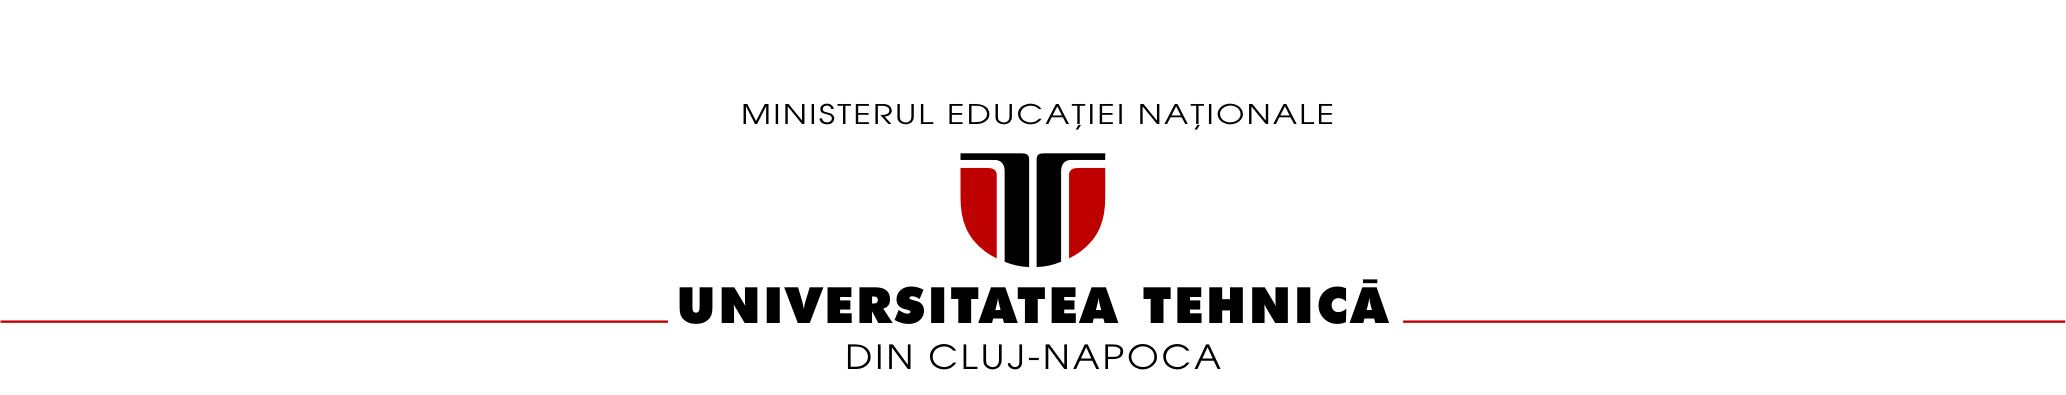
\includegraphics[width=15cm]{img/utcn.jpg}}
\newtheorem{example}{Exemplu}
\begin{document}


\section{Cerin'tele sistemului}

\subsection{Cerin'te func'tionale}

\begin{itemize}
    \item {\it Translatarea limbajului natural 'in SPARQL} - Sistemul trebuie s'a pun'a la dispozi'tie un mecanism de translatare a 'intreb'arilor din limbaj natural 'in limbaj de interogare SPARQL, precum 'si o modalitate de editare ulterioar'a a interog'arilor.
    \item {\it Interogarea\ ontologiei} -  Sistemul trebuie s'a permit'a interogarea ontologiei utiliz\ia nd limbajul de interogare SPARQL destinat ontologiilor 'si s'a ofere r'aspunsuri pe baza resurselor conceptualizate 'in baza de cuno'stin'te, utiliz\ia nd libr'aria Pellet 'si libr'aria RDFLib.
    \item {\it Permite\ vizualizarea\ elementelor\ ontologiei} - Sistemul trebuie s'a ofere capabilitatea de a expune, prin intermediul interfe'tei utilizator, a tuturor elementelor din care este constituit'a ontologia.
\end{itemize}
\subsection{Cerin'te nonfunc'tionale}
\begin{itemize}
    \item {\it Utilizabilitate} - Proiectarea sistemului 'si a interfe'tei utilizator se va face urm'arind simplitatea de utilizare. Clien'tii novici pot 'incepe utilizarea cu pu'tin instructaj asupra utiliz'arii aplica'tiei.
    \item {\it Toleran'ta\ la\ e'sec} - Sistemul este construit 'in a'sa fel 'inc\ia t, 'in cazul in care acesta e'sueaz'a 'in interpretarea intreb'arii sau pentru g'asirea unui r'aspuns, utilizatorul va fi rugat s'a repete 'intrebarea sub o alta forma sau s'a verifice interogarea.
    \item {\it Securitate} - Datele ontologiei pot fi vizualizate, fiind publice utilizatorilor, dar nu se va permite realizarea interog'arilor care pot modifica  sau altera starea acestora.
    \item {\it Explicativ} - Realizarea sistemului va 'tine cont de transparen'ta de realizare a opera'tiilor, c'at si de dreptul utilizatorului de a fi implicat 'in procesul de decizie.
\end{itemize}





\section{Validare}

Sec'tiunea de validare cuprinde o descriere a felului 'in care au fost 'indeplinte cerin'tele stabilite ale aplica'tiei. 'In sistem se realizeaz'a cu succes utilizarea limbajului natural pentru a exprima o cerin't'a. Prin intermediul unui limbaj de interogare se va interoga ontologia pentru a ob'tine r'aspunsul aferent. Sistemul implementeaz'a dou'a metode de interogare prin care utilizatorul poate s'a solicite r'aspunsul. Aplica'tia construit'a ofer'a posibilitatea de a vizualiza toate elementele ontologiei, prin intermediul unei ferestre speciale. 'In Anexa B este prezentat 'intregul set de 'intreb'ari pe care utilizatorul le poate adresa sistemului. 'In cadrul dezvolt'arii acestei aplica'tii, accentul a fost pus pe func'tionalitate, 'si mai pu'tin pe dezvoltarea unui set de 'intreb'ari extrem de cuprinz'ator. Chiar 'si 'in aceste cazuri, 'intreb'arile acoper'a cea mai mare parte a informa'tiilor ontologiei.

Prin devoltarea acestui sistem, cerin'ta nonfunc'tional'a de a avea un agent $explicativ$ este satisf'acut'a prin modul de realizat'a prin func'tionalit'a'tile alese. $Securitatea$', {\it toleran'ta\ la\ e'sec} 'si {\it utilizabilitatea} sunt cuprinse de procesul de dezvoltare.


{\bf Utilizabilitate}

Aceast'a cerin'ta este satisf'acut'a printr-o interfa'ta simpl'a, prezentat'a 'in ~\ref{fig:ui1}, ce poate fi accesat'a 'in mediul online. Datorit'a formul'arii cerin'tei 'in limbaj natural, utilizatorul nu are nevoie de training pentru utilizarea sistemului. Editarea interog'arii permite flexibilitate 'in utilizabilitate, astfel clientii mai avansa'tii pot interoga ontologia utiliz\ia nd interog'ari SPARQL. Pentru a avea o vedere de ansamblu asupra con'tinutului ontologiei, utilizatorii pot vizualiza elementele acesteia prin intermediul unei pagini prezentat'a in figura ~\ref{fig:ui2}.


\begin{figure}
    \centering
    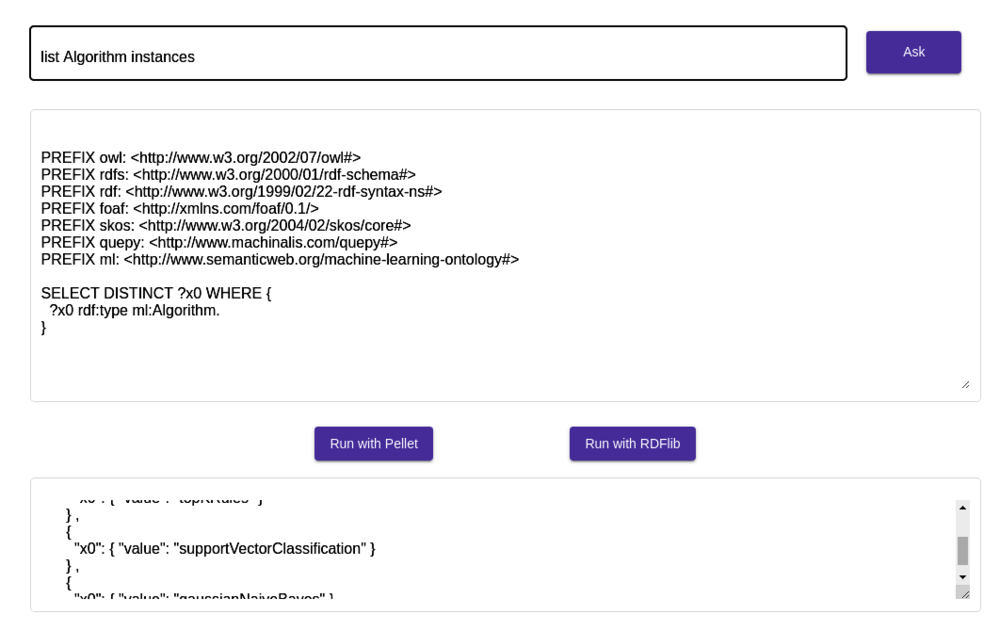
\includegraphics[width = 0.65 \linewidth]{img/pg1_cut.png}
        \caption{Pagina pentru adresarea 'intreb'arilor}
    \label{fig:ui1}
\end{figure}

\begin{figure}
    \centering
    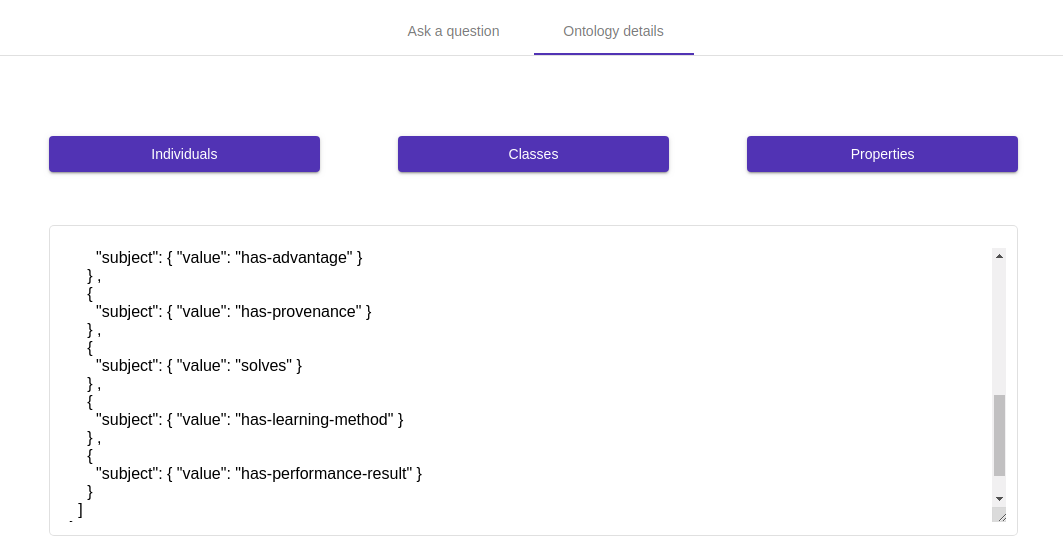
\includegraphics[width = 0.65 \linewidth]{img/ui2.png}
        \caption{Pagina pentru explorarea ontologiei}
    \label{fig:ui2}
\end{figure}


{\bf Toleran'ta la e'sec}

Pentru a permite o experien't'a c\ia t mai bun'a 'in interac'tiunea cu agentul explicativ, sistemul este implementat astfel 'inc\ia t s'a aten'tioneze utilizatorul 'in cazurile 'in care realizeaz'a opera'tii care con'tin date defectuoase. Pentru cazurile 'in care field-ul pentru 'intrebare sau field-ul pentru interogare sunt goale, butoanele sunt dezactivate 'si utilizatorul nu poate face nicio ac'tiune. Se trateaz'a 'si cazurile 'in care 'intrebarea nu este formulat'a corect sau interogarea SPARQL nu este valid'a, pentru aceste situa'tii sistemul return'and aten'tion'ari pentru a semnala provenien'ta e'secului.

{\bf Securitate}

Pentru 'indeplinirea obiectivului de securitate am considerat restric'tionarea interog'arilor SPARQL la opera'tii de vizualizare. A'sadar, utilizatorul nu poate s'a realizeze opera'tii de inserare, 'stergere sau alte modific'ari asupra datelor. De asemenea, accesul la ontologie este restric'tionat, caz 'in care clientul poate numai s'a vizualizeze numai clasele, indivizii 'si rolurile con'tinute de ontologie.  

{\bf Explicativ}

Cerin'ta ca sistemul s'a fie explicativ este 'indeplinit'a prin introducerea pasului suplimentar 'in care utilizatorul poate s'a vizualizeze 'si s'a editeze interogarea SPARQL, astfel 'in'teleg\ia nd modul de extragere al r'aspunsului. Prin acest fapt, sistemul nu este considerat o cutie neagr'a 'in care intrarea este o 'intrebare, iar ie'sirea este un r'aspuns. Utilizatorul poate s'a foloseasc'a 'si pagina pentru solicitarea detaliilor ontologiei pentru a 'intelege provenien'ta r'aspunsului.


\end{document}